\chapter{Visualisation implementation of the Improved Kepler Visualisation Tool
(IKVT)}\label{C:sd}
This chapter discusses the implementation of the visulisation using the designs
discussed in the previous chapter to fulfill the requirements for this project.
It details the tools used, the deliverable features
produced, and the problems encountered. 

\section{Tools and Artifacts Used}
\subsection{Keyboard \& Mouse System}
In addition to Processing there was an additional opensource
library required for effective user interface components called ControlP5
\cite{controlp5}. This library provides customisable and intuitive

user interface components. It allows for the creation of visually appealing and
precisely
laid out interactive GUI components.

\subsection{Microsoft Kinect System}
For the Microsoft Kinect version of IKVT two additional libraries were required
to integrate the Kinect sensor
with Processing, these were:
\begin{enumerate}
 \item NITE \cite{nite}
 \item SimpleOpenNi \cite{simpleopenni}
\end{enumerate}
These libraries provided drivers to run the Kinect sensor in Processing
(SimpleOpenNi) as well
as basic gesture recognition and body tracking (NITE). However these libraries
were
opensource options due to the official Microsoft Kinect SDK not being compatible
with
Processing. This meant the gesture recognition was not as user friendly or
effective as the
official libraries. The effect of this was that the gesture tracking used in the
system had to be created sup-optimally from the opensource libraries which took
more time and resources. 

\section{Implementation of IKVT}

IKVT displays all 2234 exoplanets
in the Kepler exoplanets dataset \cite{dataset}. Each of these exoplanets are
represented as coloured
ellipses, of which the colour and size are representative of the exoplanets
temperature and size respectively. IKVT displays all of these exoplanets as if
they are orbiting a single star which in reality would result in planetary
collisions but in the visualisation provides users with a way to effectively
make observations and comparisons about each of the exoplanets in a single
view. 

There are two panels that make up the visualisation, the visualisation panel,
and the control panel. The visualisation panel is where the exoplanets
are displayed as well as a text boxes describing the state of the visualisation
to
keep the user informed. The control panel contains all of the interactive
components that the user can use to change the state of the visualisation. The
components it contains are; two text areas that cane be used interchangeably to
display information about selected planets, four range sliders shown in Figure 
\ref{fig:sliders} that are used to
filter the exoplanets as discussed previously, and eight buttons to toggle the
state of the visualisations. These buttons are "Sort by KOI", "Sort by Temp",
"Sort by Size", "Sort by ESI", "Change View", "Suns Habitable Zone", "Pause",
and "Unsort" as shown in Figure: \ref{fig:buttons}. 

\begin{figure}[H]
  \centering
      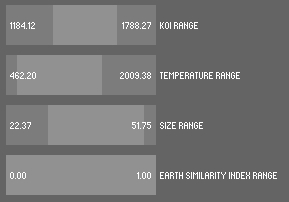
\includegraphics[width=0.6\textwidth]{images/sliders.jpg}
  \caption{Panel of interactive range sliders}
  \label{fig:sliders}
\end{figure}

\begin{figure}[H]
  \centering
      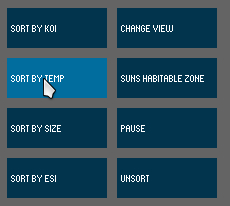
\includegraphics[width=0.6\textwidth]{images/buttons.jpg}
  \caption{Panel of interactive buttons}
  \label{fig:buttons}
\end{figure}

Detailed information can be accessed about each exoplanet by clicking on them in
the main visualisation window to
make a selection. To do this a user can click on any of the orbiting exoplanets.
The effect of this selection is that a text box will have further textual
information about the selected exoplanet appended to it. In addition to this
users have the option of clicking a button labeled  as ``Compare'', This allows
the user the option to select another exoplanet so that its information is
appended to a second text area. This can be seen in Figure \ref{fig:textBoxes}. 
\begin{figure}[H]
  \centering
      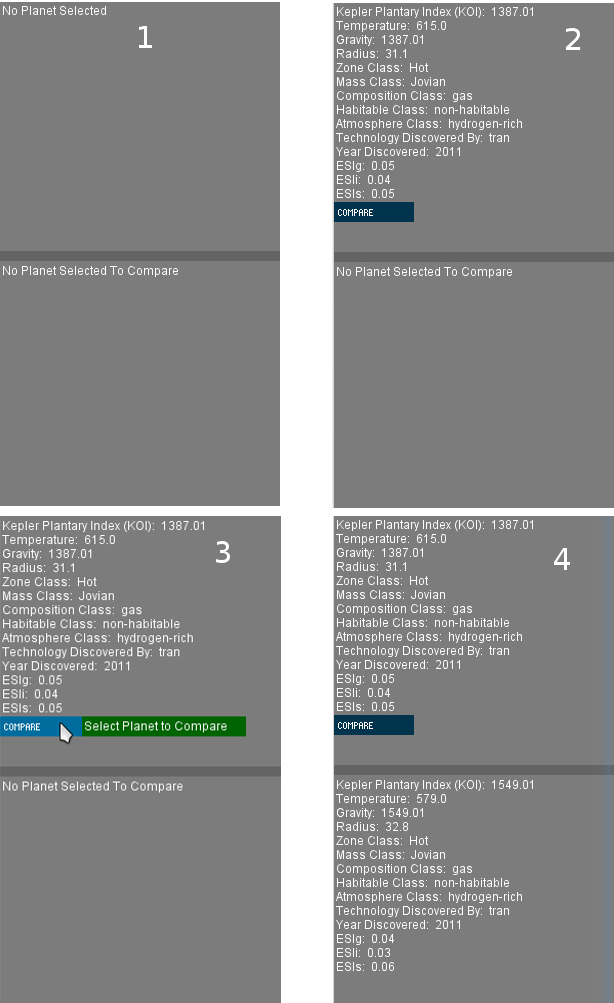
\includegraphics[width=0.7\textwidth]{images/textBoxes.jpg}
  \caption{Text boxes in each possible state}
  \label{fig:textBoxes}
\end{figure}
When a user is unable to accurately select an
exoplanet due to clustering or
overlapping of exoplanets they can move the camera around in space to gain a
better viewing position with which to make their selection. If this is not
enough, the user can use a set of range selectors to filter the exoplanets
displayed, as shown in Figure \ref{fig:zoomFilter}. The attributes that can be
filtered by are the Kepler Object of Interest number (KOI),
temperature, size, and Earth Similarity Index (ESI). These filters allow for
users to fine tune the exoplanets they wish to view, thus allowing them to work
with small multiples rather than the entire dataset. A further effect of using
these filters is that a zooming effect occurs as exoplanets are filtered out.
This zooming occurs each time the filters are changed as the exoplanets spread
out vertically which allows more space between them to make selections.

\begin{figure}[H]
  \centering
      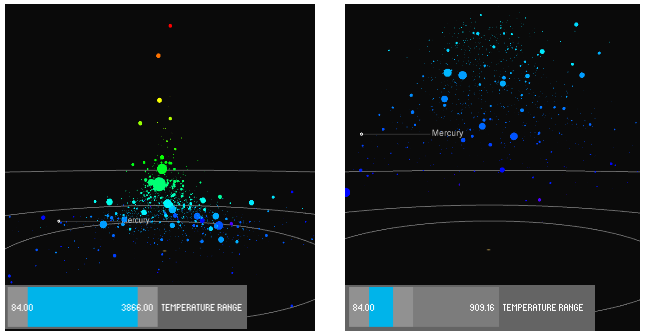
\includegraphics[width=0.8\textwidth]{images/zoomFilter.png}
  \caption{TODO~}  
    \label{fig:zoomFilter}
\end{figure}

The existing Kepler Visualisation Tool allowed users to sort the exoplanets on
the Y axis by their temperature and size. In IKVT this has been extended to
allow sorting by Kepler Object of Interest number (KOI) and Earth Similarity
Index (ESI) as shown in Figure \ref{fig:ESIKOI}.


\begin{figure}[H]
  \centering
      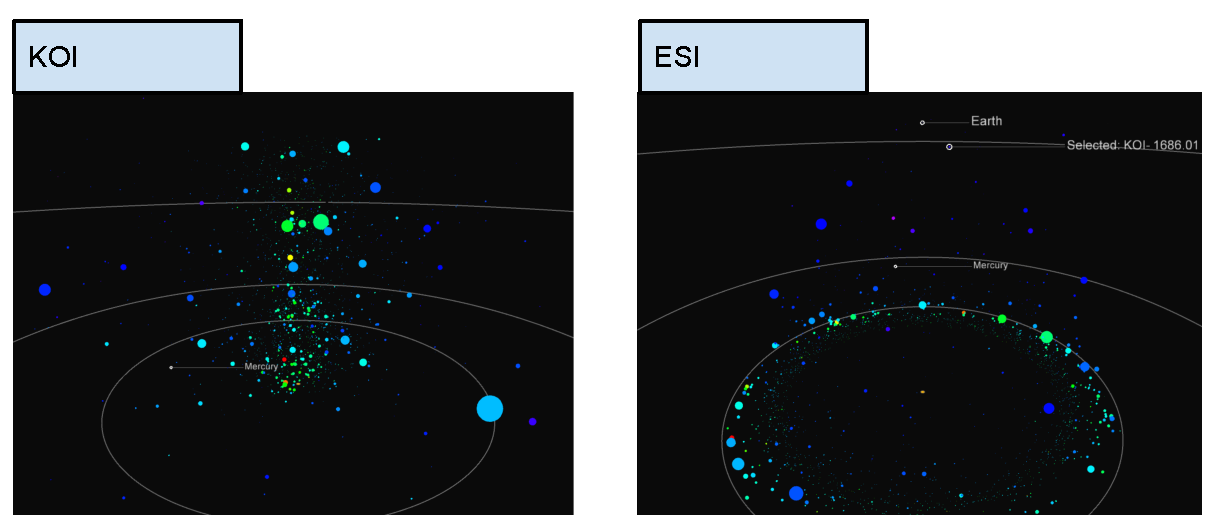
\includegraphics[width=1\textwidth]{images/ESIKOI.pdf}
  \caption{TODO~}  
    \label{fig:ESIKOI}
\end{figure}

When a exoplanet is selected it is important that the user gets feedback about
what they have done. In IKVT this happens in the form of the selected exoplanet
becoming larger and a white outlining ring expanding out to encircle it. In
addition to this a label appears to the right of the exoplanet and states the
Kepler Object of Interest number (KOI). 

\begin{figure}[H]
  \centering
      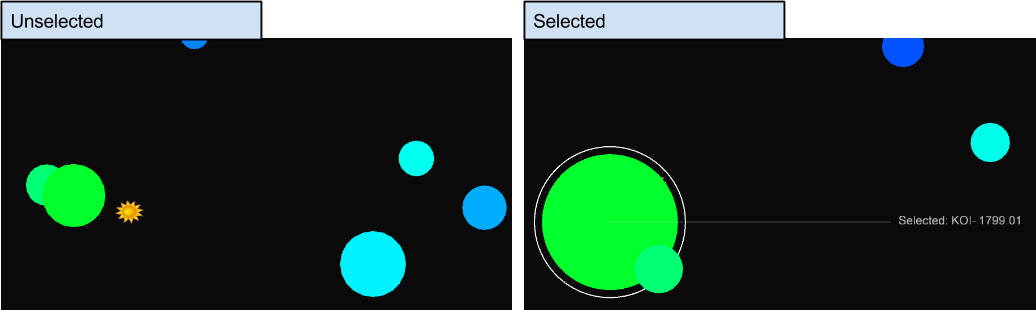
\includegraphics[width=1\textwidth]{images/selectedPlanet.jpg}
  \caption{TODO~}  
    \label{fig:selectedPlanet}
\end{figure}

Another effect of a user making a selection is that all exoplanets that share
the same star as the selected exoplanet also become highlighted in the
same way as outlined above. The only difference is that in the label to the
right
of each exoplanet the message now informs the user that it has the ``Same
Star'' as displayed in Figure \ref{fig:sameStar}.

\begin{figure}[H]
  \centering
      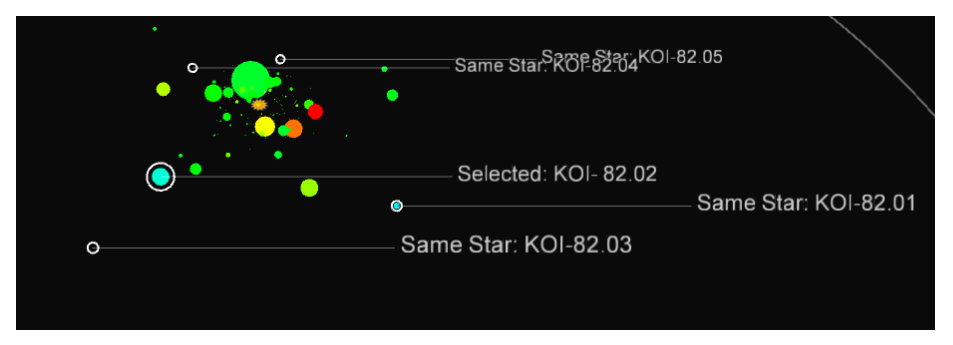
\includegraphics[width=1\textwidth]{images/sameStar.png}
  \caption{TODO~}  
    \label{fig:sameStar}
\end{figure}


To display the Goldilocks zone of selected exoplanets coloured rings appear to
display the habitable
and inhabitable zones of the star. Each time a new planet is selected the
coloured rings change to represent the newly selected exoplanets star, this can
be seen in Figure
\ref{fig:habitable}. In addition to the coloured rings the selected planet also
becomes highlighted
and the rest become transparent making it stand out to help users understand
whether it is in a habitable zone or not.

\begin{figure}[H]
  \centering
      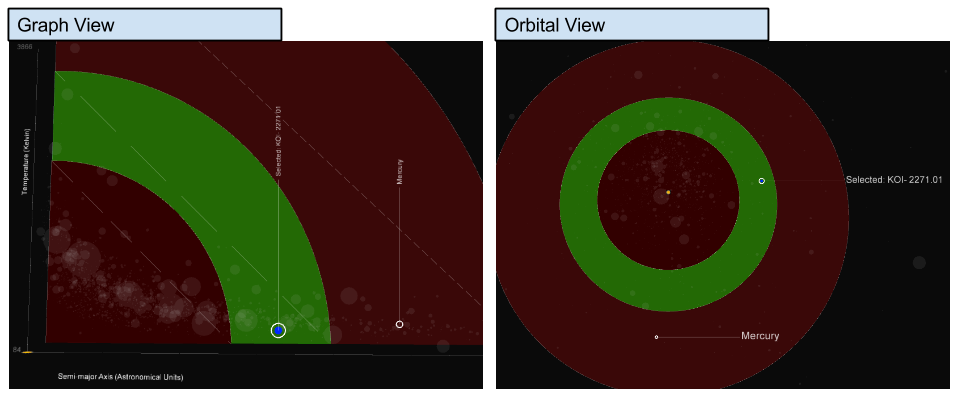
\includegraphics[width=1\textwidth]{images/habitable.png}
  \caption{TODO~}  
    \label{fig:habitable}
\end{figure}

Each of these implemented elements need to be visually apparent and intuitive to
use to ensure that the system can be
easily used without prior experience. This is done by providing clearly
labeled interactive elements and tooltips explaining what they
do as in Figure \ref{fig:tooltip}. These tooltips are widely used as a method of
informing a
user about the purpose of an item by hovering over it removing the need to
click on a button to discover its effect.

\begin{figure}[H]
  \centering
      
\includegraphics[width=0.8\textwidth]{images/tooltip.jpg}
  \caption{Tooltip on hover}
  \label{fig:tooltip}
\end{figure}

Due to the need for effective user interaction with the visualisation, a window
is required to house all of the components discussed above. Having this window
spatially separated from the main visualisation window means that users will not
be drawn away from the visualisation by overlapping and intrusive controls. Each
of the controls discussed above are included in this panel as shown below in
Figure \ref{fig:nav}.

\begin{figure}[H]
  \centering
      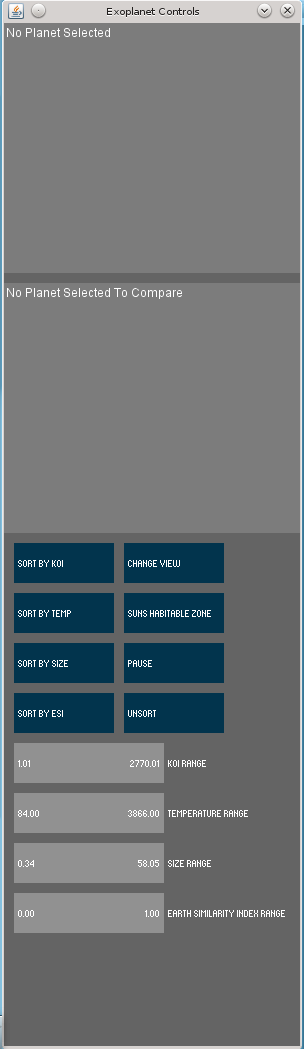
\includegraphics[width=0.3\textwidth]{images/nav.png}
  \caption{Navigation Panel Overview}
  \label{fig:nav}
\end{figure}

At first the visualisation was laid out so that the interaction panel took up a
300 pixel strip along the bottom of the screen with the main visualisation
window
taking up the rest of the space as in Figure \ref{fig:layoutOld}.
 This was found not to be suitable as the majority of the interaction and
animation of visualisation elements occurs
in the center of the window which this layout did not effectively utilise as it
caused a low aspect ratio that made the top and bottom of the visualisation to be
cut off. It
was more effective to use two vertical columns as in Figure \ref{fig:layoutNew},
to view and control the visualisation. This is because
the higher aspect ratio allowed more of the content to be seen on the
screen at once, thanks to the fact that the majority of computer screens have a
wide aspect ratio. As you can see by comparing the two figures, Figure
\ref{fig:layoutNew} cuts off less of the visualisation and so is a more suitable
choice.

\begin{figure}[H]
  \centering
      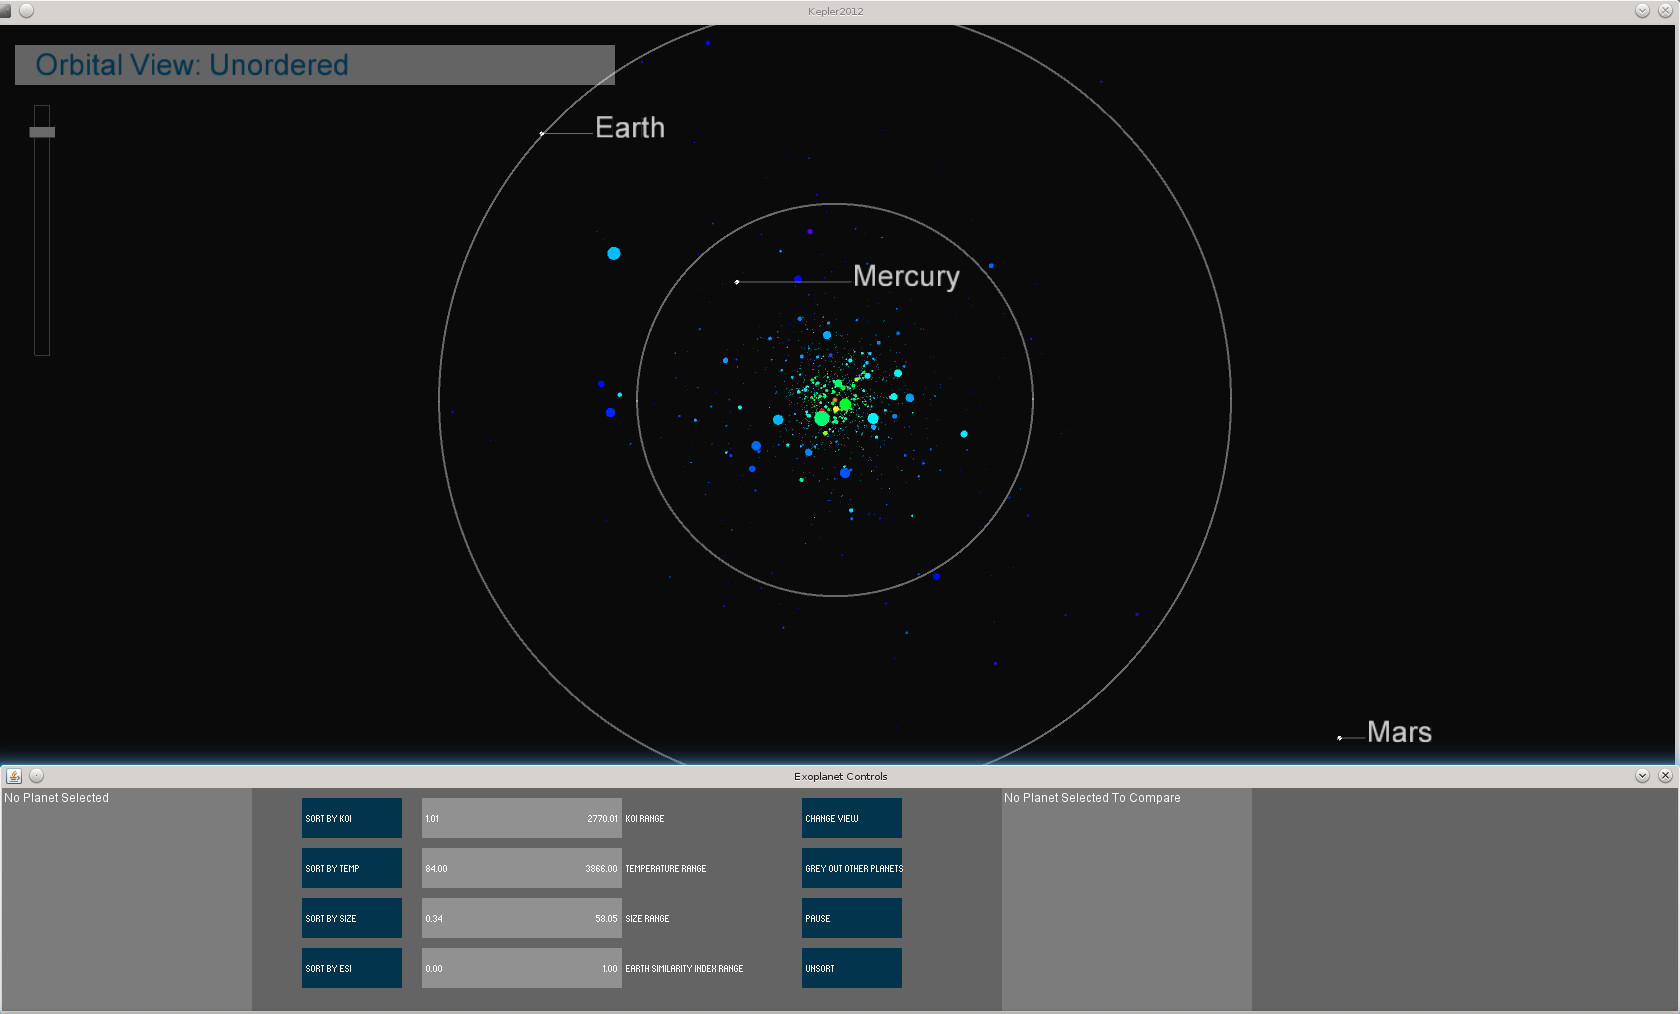
\includegraphics[width=0.8\textwidth]{images/layout_horizontal.jpg}
  \caption{Original Horizontal Layout}  
    \label{fig:layoutOld}
        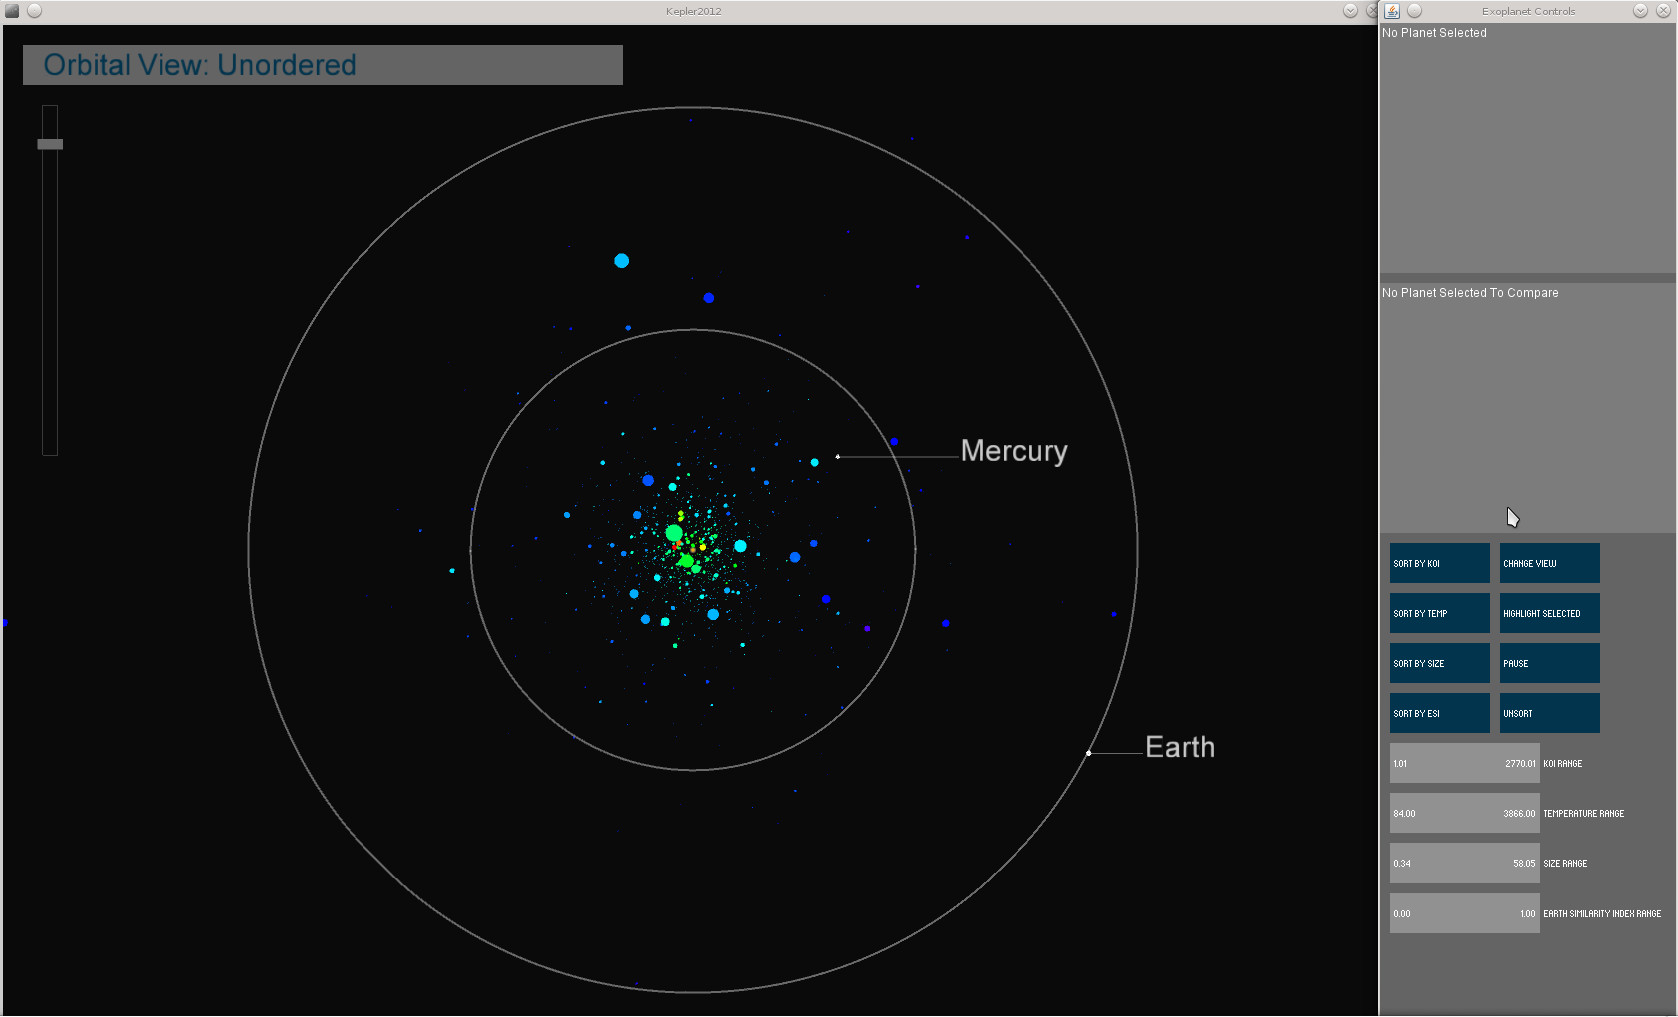
\includegraphics[width=0.8\textwidth]{images/layout_vertical.jpg}
  \caption{Improved Vertical Layout}
  \label{fig:layoutNew}
\end{figure}

The Kinect Sensor system uses all of the features discussed above and extends it
by incorporating in gesture based control by utilising a Microsoft Kinect
sensor. Incorporate these gesture based controls was completed by specifying
gestures are detected by the visualisation which in turn modifies its state. As
shown in the solution design stage there were eight gestures that were needed
for the visualisation, each of which was implemented as described below
\begin{enumerate}
 \item[1.] default cursor, hand is at rest or hovering over a planet
 
\begin{figure}[H]
  \centering
      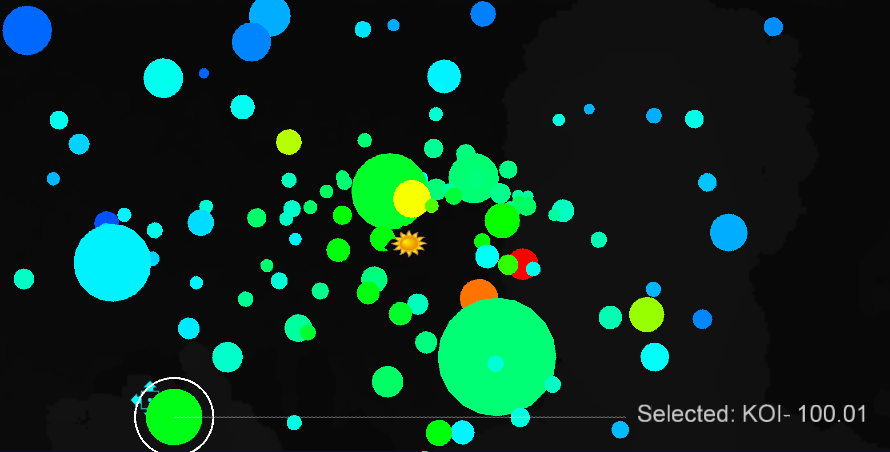
\includegraphics[width=0.8\textwidth]{images/select.PNG}
  \caption{TODO}
  \label{fig:left}
\end{figure}

 \item[2 \& 3.] panning up, hand is raised or panning down, hand is lowered
 \begin{figure}[H]
  \centering
      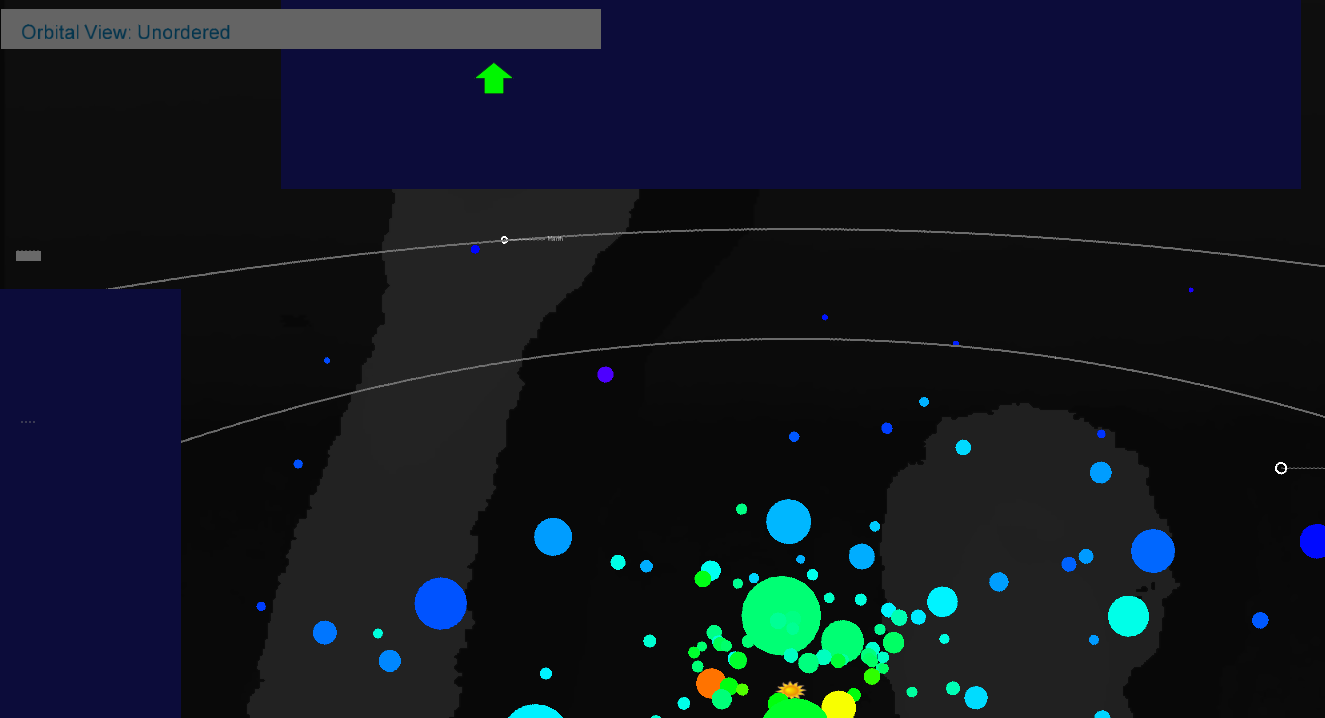
\includegraphics[width=0.8\textwidth]{images/up.PNG}
  \caption{TODO}
  \label{fig:up}
\end{figure}
 
 \item[4 \& 5.] rotating left, hand is to the left or rotating right, hand is to
the right
 
\begin{figure}[H]
  \centering
      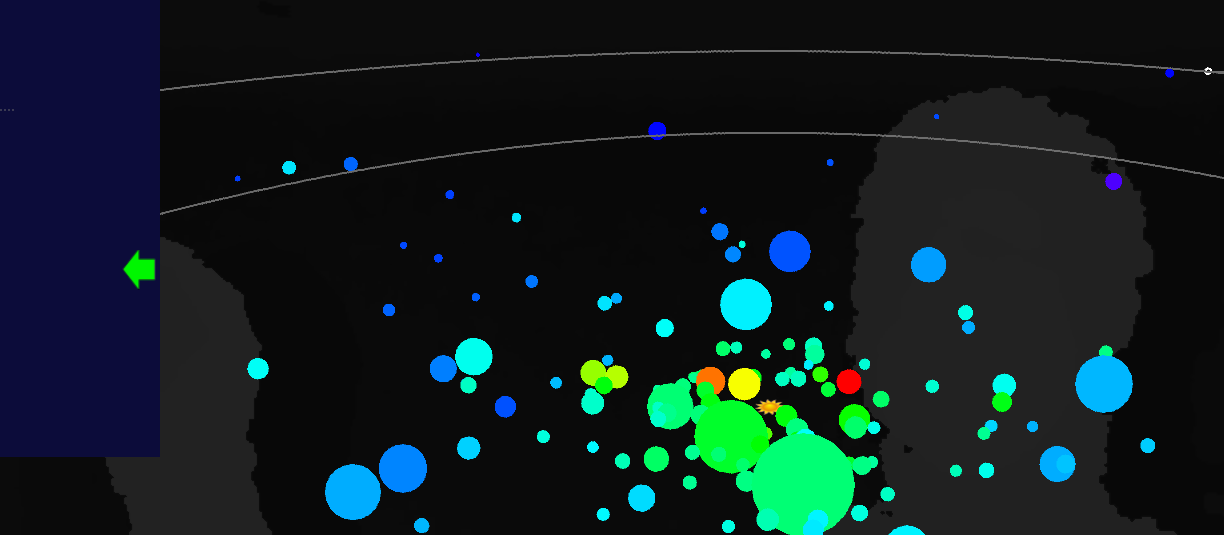
\includegraphics[width=0.8\textwidth]{images/left.PNG}
  \caption{TODO}
  \label{fig:left}
\end{figure}

 \item[6.] zooming in, hand is pressed forward
 \begin{figure}[H]
  \centering
      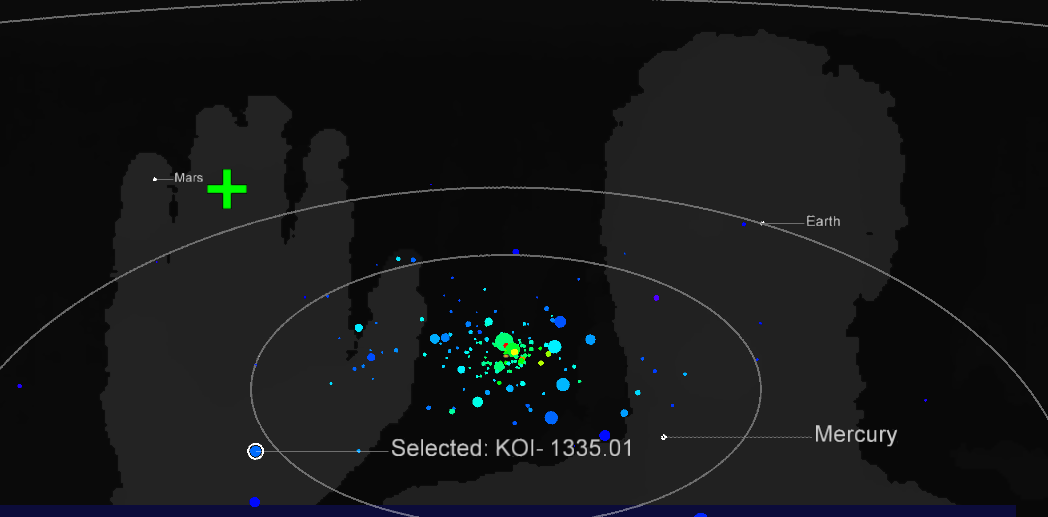
\includegraphics[width=0.8\textwidth]{images/in.PNG}
  \caption{TODO}
  \label{fig:in}
\end{figure}

 \item[7.] zooming out, hand is pulled backwards
 
\begin{figure}[H]
  \centering
      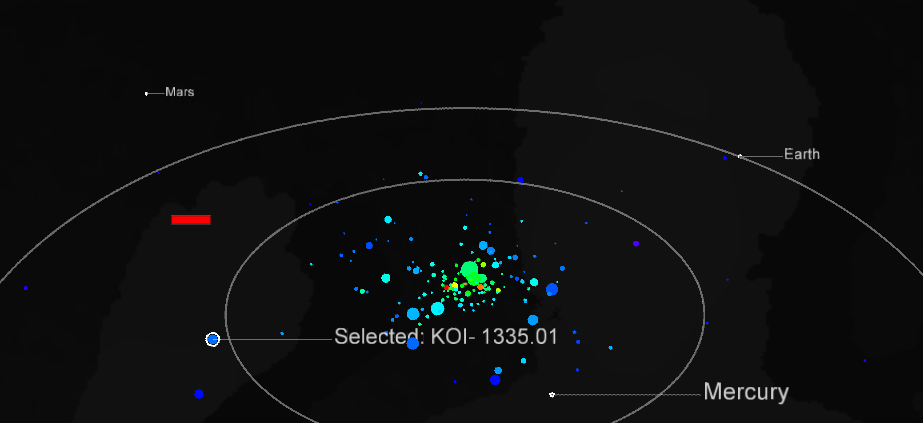
\includegraphics[width=0.8\textwidth]{images/out.PNG}
  \caption{TODO}
  \label{fig:out}
\end{figure}

\end{enumerate}

In addition to this, the screen displays the user in relation to the
the visualisation, this is done by displaying a transparent outline of
the user in the background of the visualisation as can be seen in the above
figures. This is important as it gives the user a way to infer where they are
gesturing and as a way to show them that they are being detected by the system.
\\\\
Each of the features discussed were implemented using the designs created in
Chapter \ref{C:sd}: Solution Designs to fulfill the functional requirements.
The visualisation IKVT that was created can successfully display planetary
information to convey knowledge to users (Requirement 1), allow exoplanets to be
compared against one another (Requirement 2), order exoplanets by their ESI and
by their KOI (Requirement 3), allows users to define ranges of planetary
attributes to filter which planets are displayed (Requirement 4), and view the
habitable zones of stars in
relation to the planets orbiting them (Requirement 5). These functionalities
are evaluated in the next chapter to ensure that they successfully fulfill the
functional requirements as previously stated, as well as the non functional
requirements that emphasises usability for users.




\section{Problems encountered}

As this project builds upon a previous system, much of the existing code and
execution flow needed to be modified. This required understanding of how the
system was originally built and designed. Because this system did not have any
unit or integration tests, going ahead without a comprehensive knowledge of the
core functionality would be have led to ineffective planning and errors being
introduced into the system. To address this extra time and resources were
allocated to the requirements analysis and solution design stages of the
project.
\\\\
%Making use of tall of the data
Due to the number of elements that needed to be displayed on screen at any one
time (ie 2234 exoplanets), the load placed on a system is very high due to the
need to render 2234 eclipses to represent the planets. This uncovered a bug in
the Processing library in which the memory use of the visualisation would
periodically increase until it crashed due to an Out of Memory Exception. After
much experimentation of how to overcome this issue, I discovered that rather
than trying to render a native ellipse shape in processing, if I instead
rendered
a Scalable Vector Graphic this bug would not manifest. 
\\\\
Using the Processing framework meant using a non commercial IDE that is not
completely robust, for example when undoing multiple times in a row the file
being
modified would periodically become corrupted by lines of code being taken away
or inserted into the wrong locations. The solution to this issue was to ensure
that any changes were committed regularly to my repository on Github
\cite{github}. Doing this meant that if at any time a file became corrupted the
incorrect changes could be easily compared against the previous commit and
manually fixed. Any bugs found were reported in
the hopes that people using Processing in the future wouldn't need to address
them.
\\\\
The libraries used for gesture detection with the Kinect sensor were opensource
as this was the only way to get it to work with Processing. These open source
libraries did not have the functionality, documentation, and support that the
real Software Development Kit (SDK) that is available from Microsoft would have
had. Whilst this was not a roadblock in terms of development it did mean that
more time was required for research and experimentation during implementation.
\\\\

